\documentclass[9pt]{beamer}
\usepackage[utf8]{inputenc}
\usepackage[spanish]{babel}
\usepackage{newcent}

\usetheme{Warsaw}
\setbeamertemplate{footline}[frame number]

\author{Gabriel Sanhueza}

\title[JHawanet Framework]{Software para la optimización de redes de distribución de agua potable}
\subtitle{``JHawanet Framework''}
%\setbeamercovered{transparent} 
%\setbeamertemplate{navigation symbols}{} 
\titlegraphic{\includegraphics[height=1.5cm]{utalca1.eps}}
 
\institute [Universidad de Talca]{Defensa de Título\\ Universidad de Talca \and Profesores guías\\ Jimmy Gutiérrez Bahamondes \\ Daniel Mora Melia}

\date{Agosto, 2020}



\begin{document}

    \frame{\titlepage}

    \subsection{Operadores de Selección}
    \begin{frame}
        \frametitle{Operadores de Selección}                       
        \textit{Tournament Selection}
        \begin{figure}
            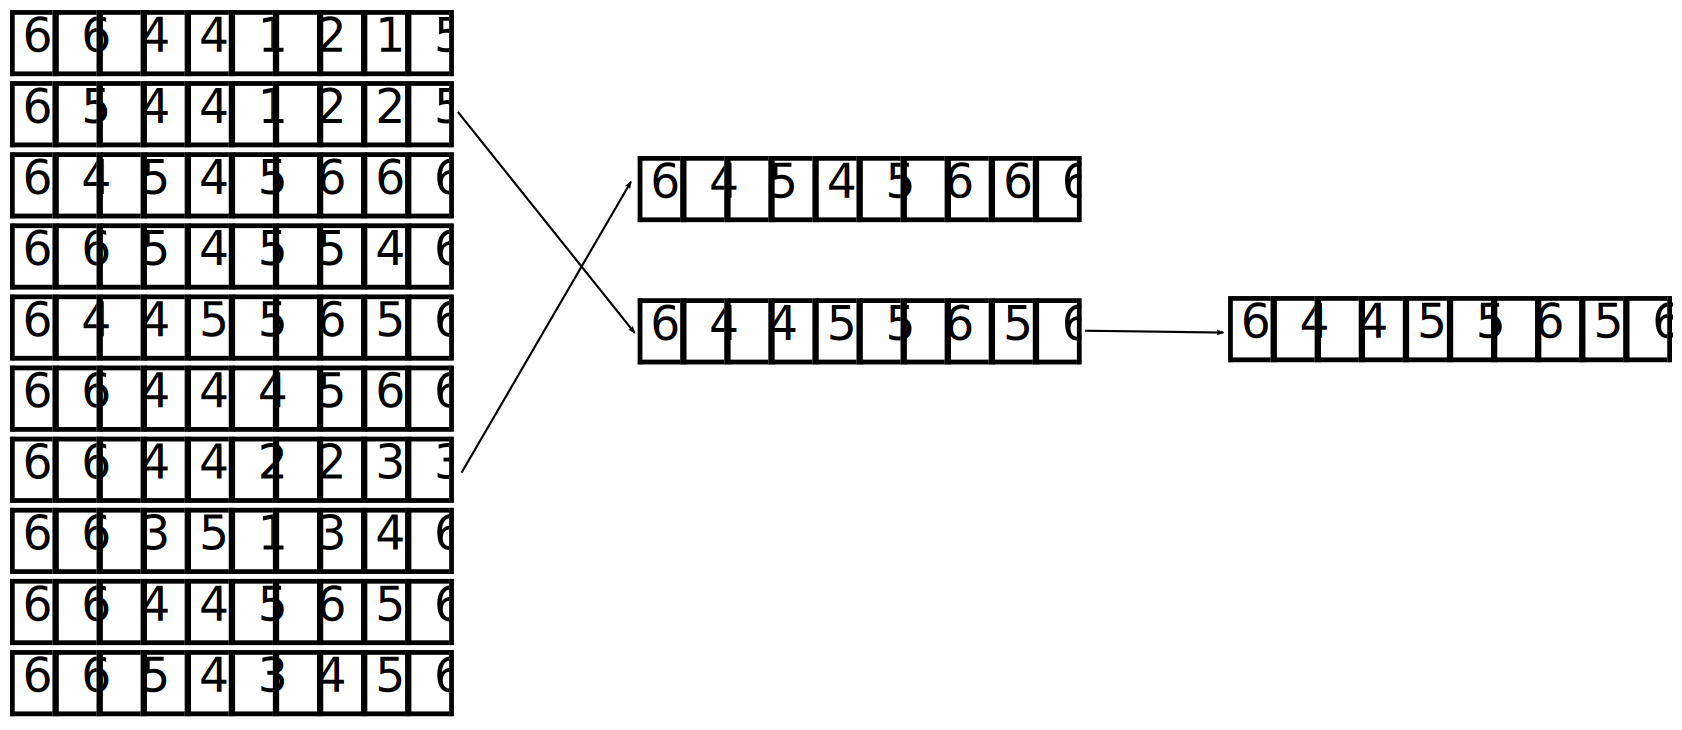
\includegraphics[width=\textwidth]{assets/Anexo/TournamentSelection.eps}
        \end{figure}
    \end{frame}
    \begin{frame}
        \frametitle{Operadores de Selección}
        \textit{Uniform Selection}
        \begin{columns}
            \column{0.5\textwidth}
            $$p_{max} = \frac{\beta}{N_c}$$
            $$p_{min} = \frac{2-\beta}{N_c}$$
            $$1.5 <= \beta <= 2$$             
            $$p_{i} = p_{min} + (p_{max} - p_{min}) \times \frac{N_c - i}{N_c - 1}$$                  
        
            \column{0.5\textwidth}
            \begin{figure}
                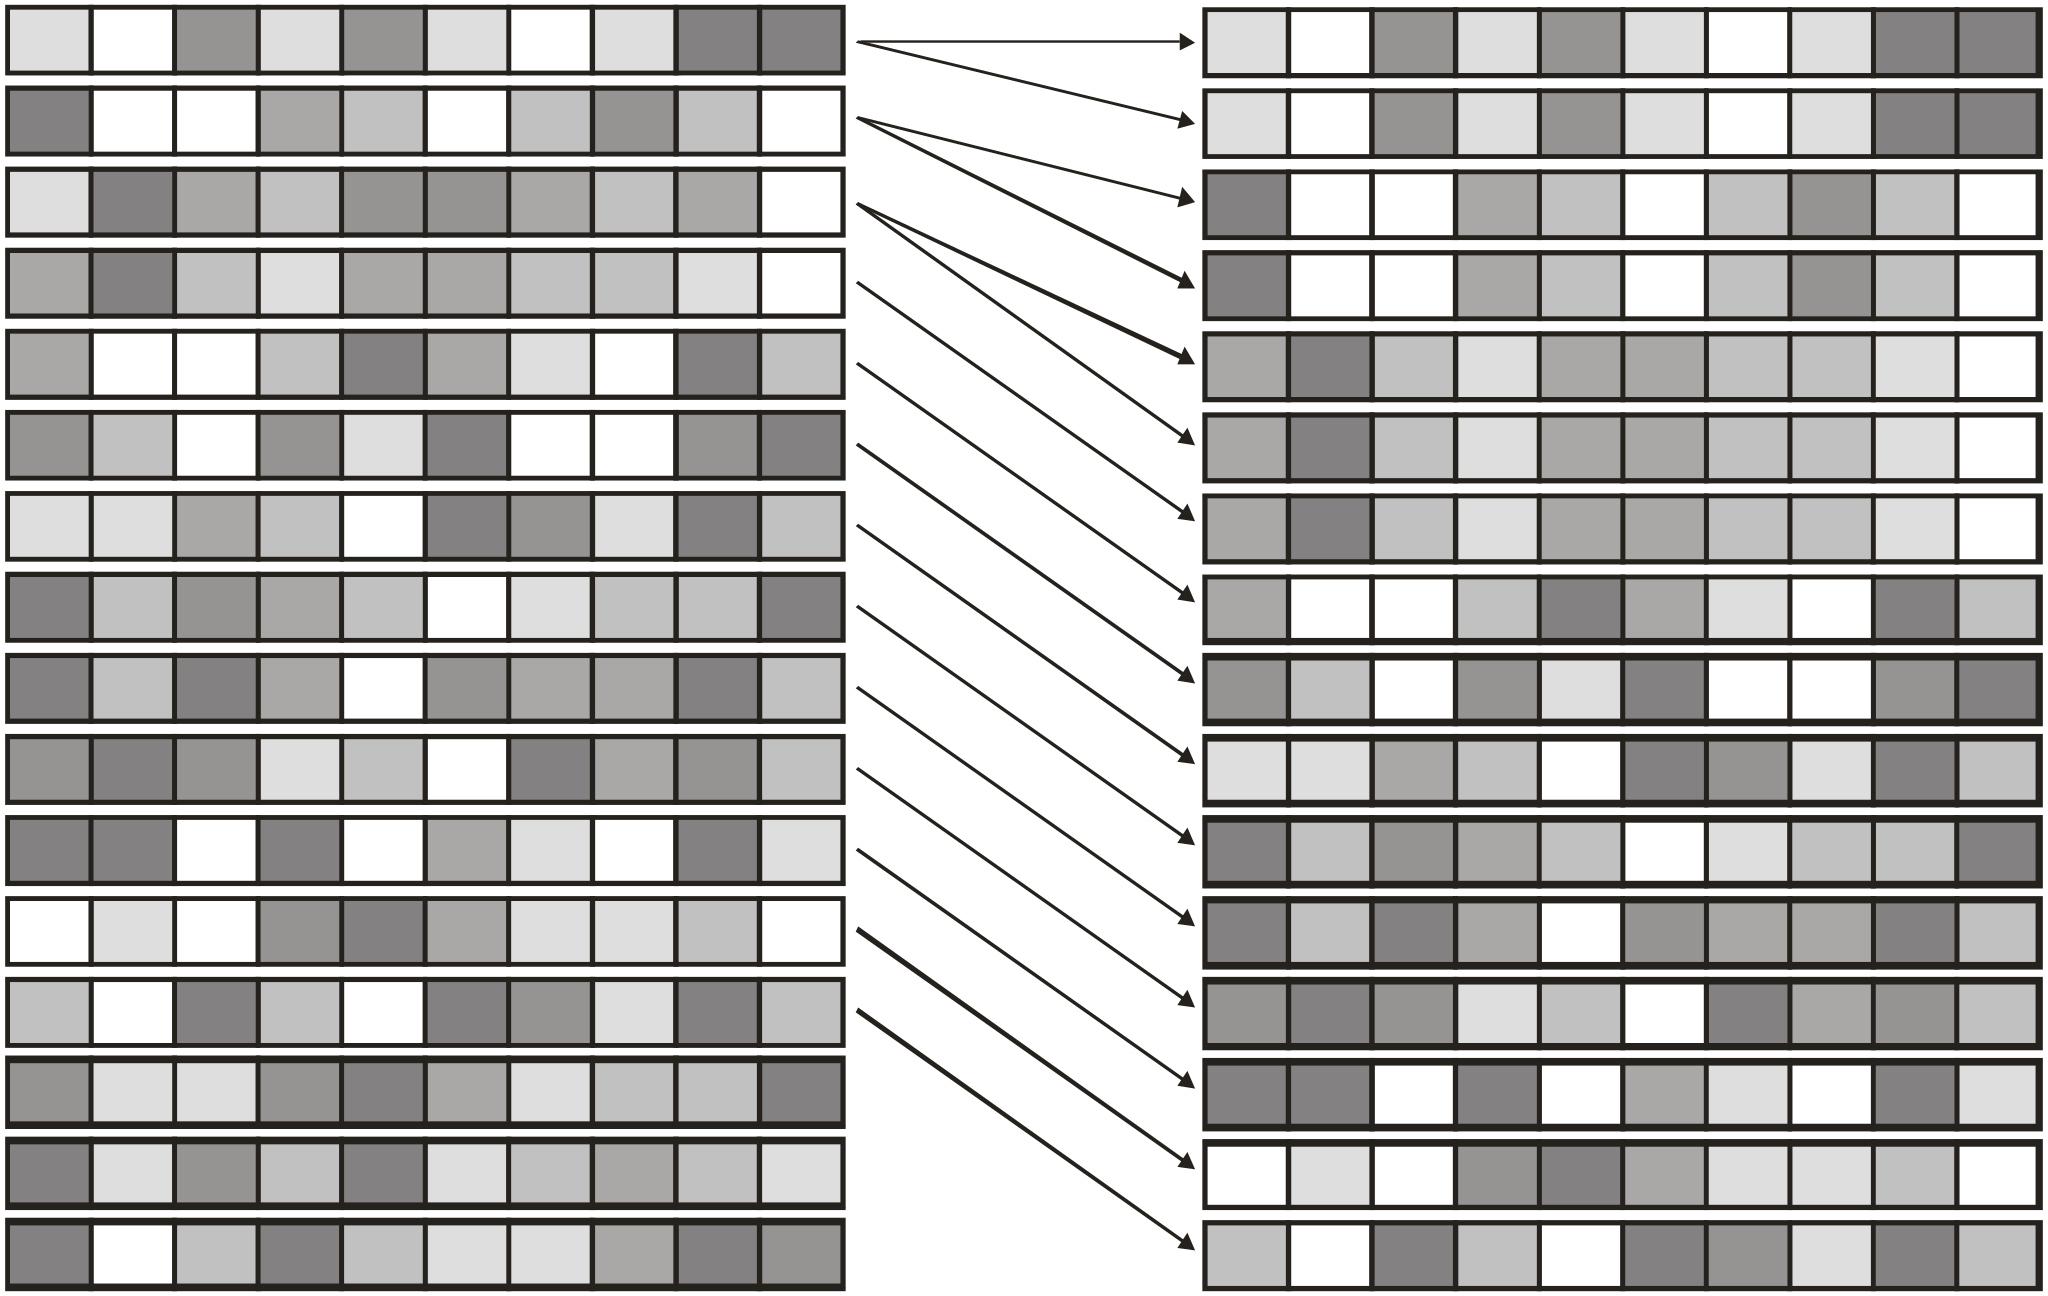
\includegraphics[width=\textwidth]{assets/Anexo/UniformSelection.eps}
            \end{figure}
        \end{columns}

    \end{frame}

    \subsection{Operadores de Cruzamiento}
    \begin{frame}
        \frametitle{Operadores de Cruzamiento}
        \textit{SinglePointCrossover}

        \begin{figure}
            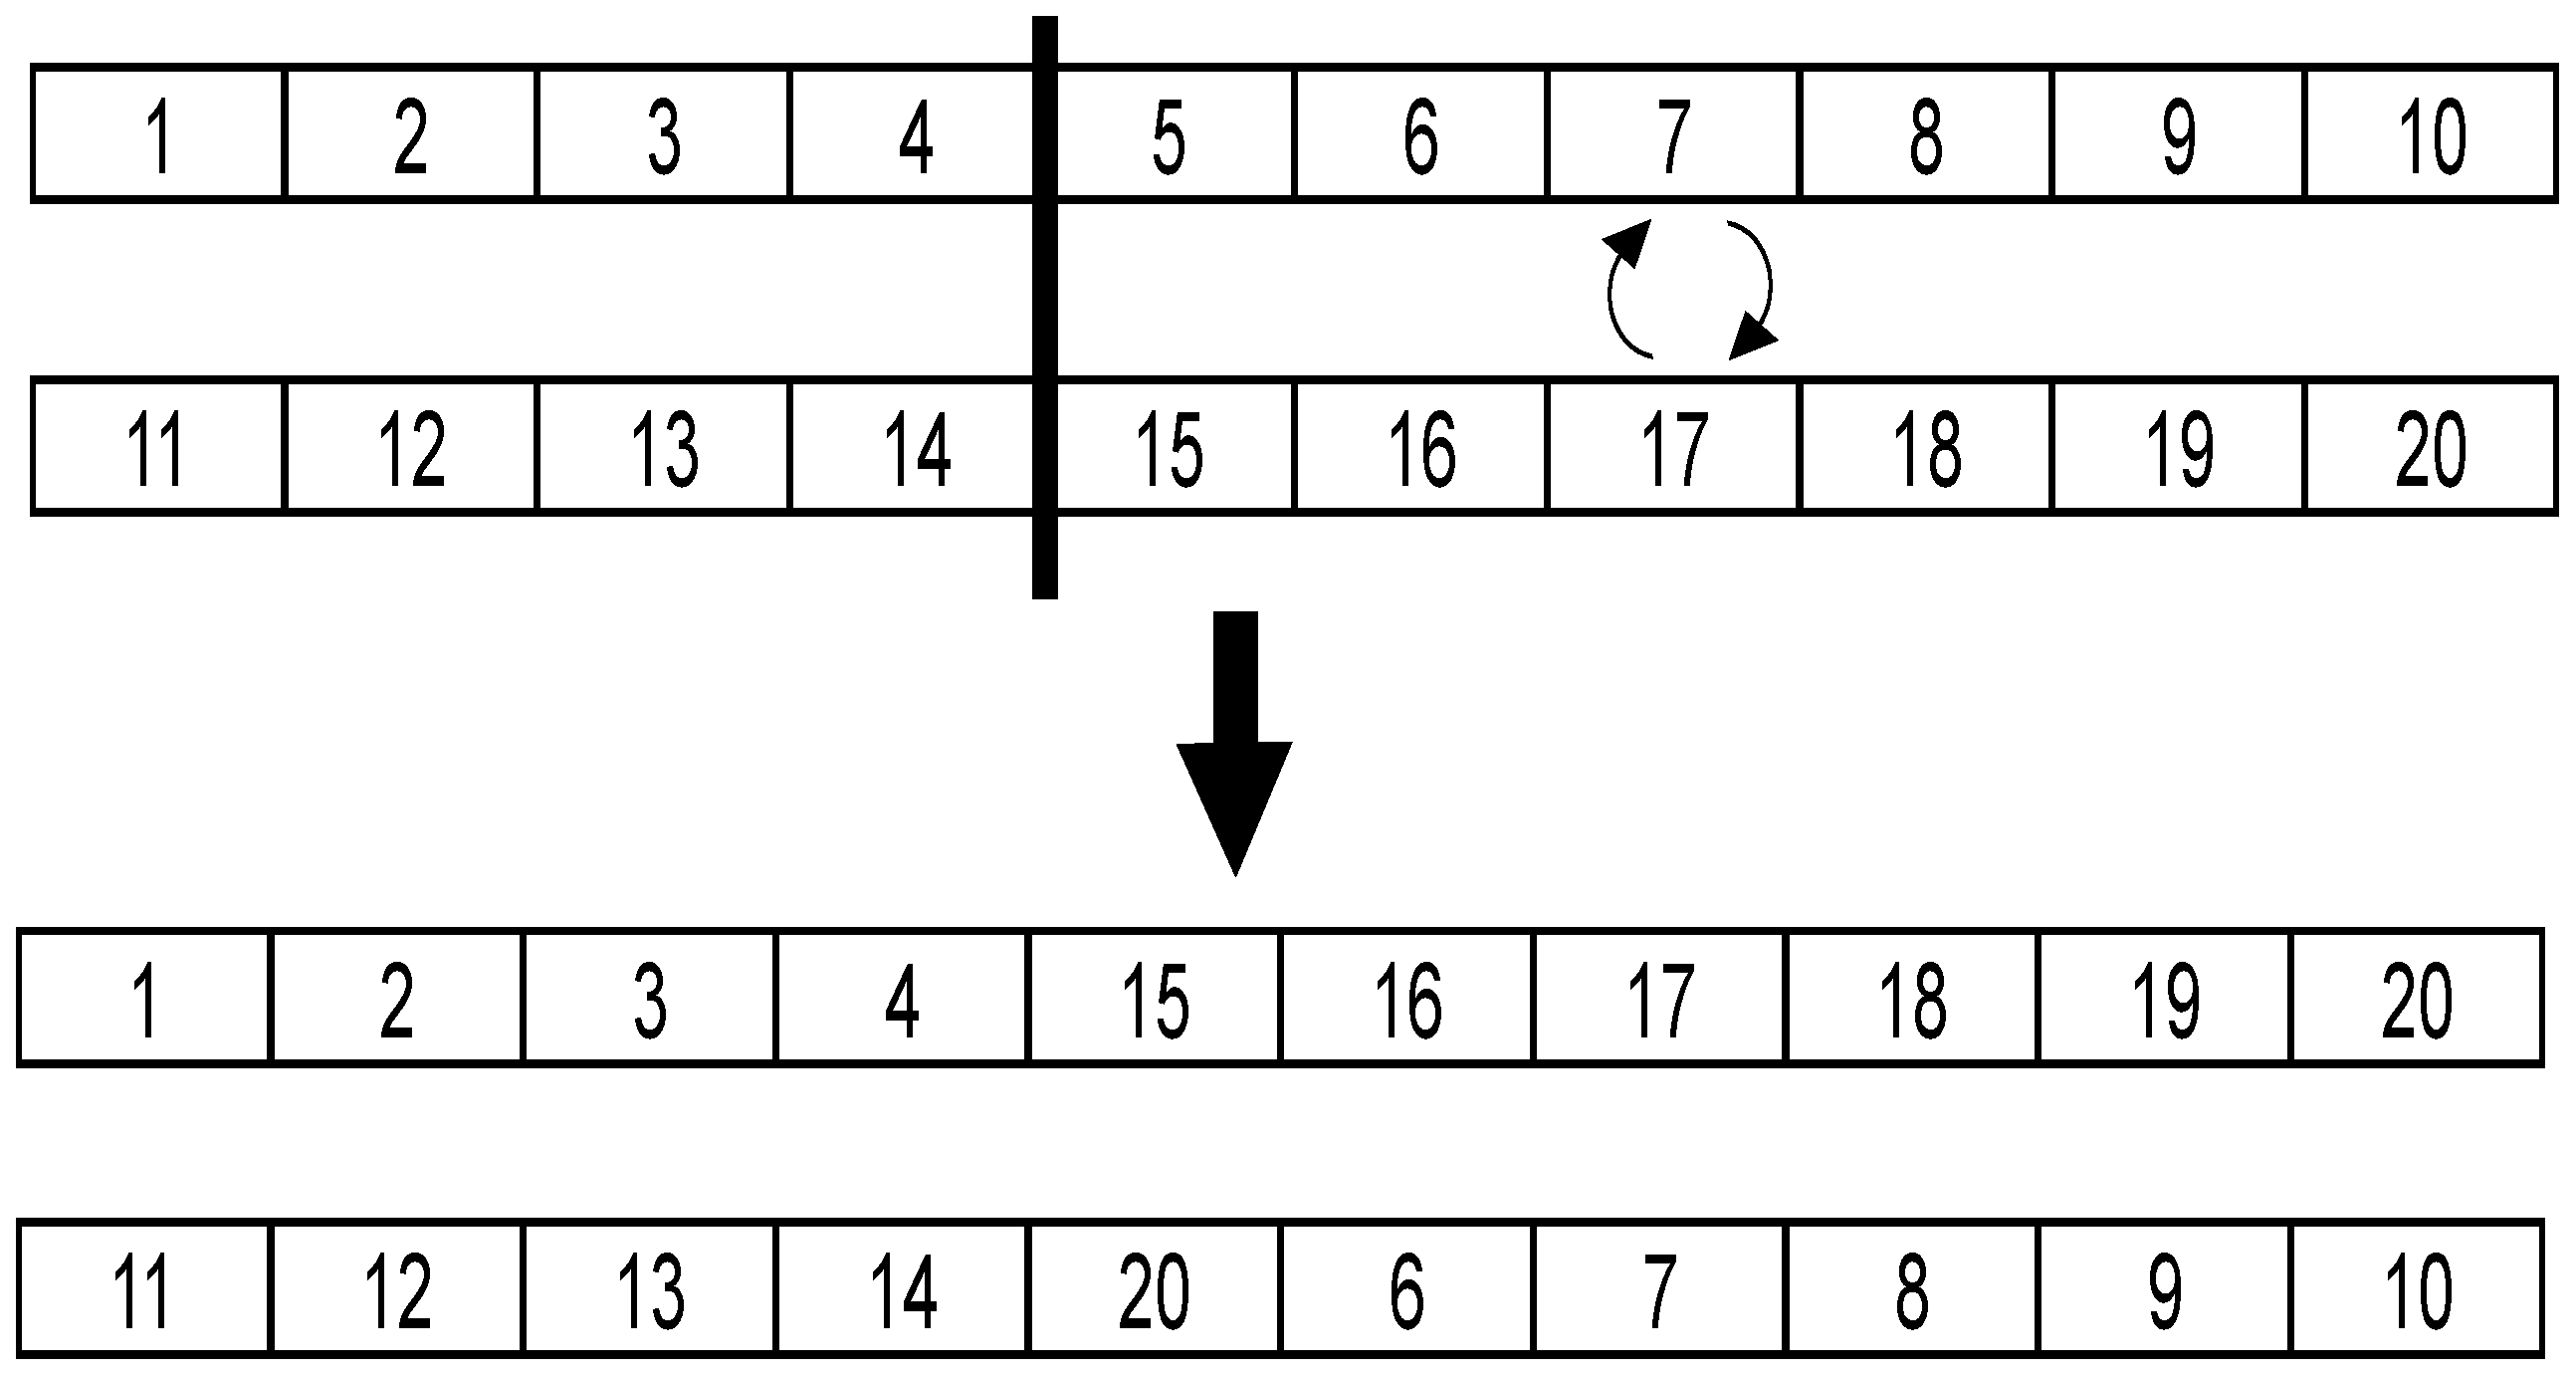
\includegraphics[width=\textwidth]{assets/Anexo/Crossover.eps}
        \end{figure}

    \end{frame}

    \begin{frame}
        \frametitle{Operadores de Cruzamiento}
        \textit{SBXCrossover}
        
        $$
        \begin{cases} 
            \beta_q=\sqrt[d_i+1]{r\alpha} & \text{si $r\leq \frac{1}{\alpha}$} \\ 
            \beta_q=\sqrt[d_i+1]{\frac{1}{2-r\alpha}} &  \text{si $r > \frac{1}{\alpha}$}
        \end{cases}
        $$
        
        
        \begin{columns}
            \column{0.5\textwidth}
            $$\beta = 1 + 2\frac{y_1-yL}{y_2-y_1}$$
            $$\alpha = 2 - \frac{1}{\beta^{di+1}}$$
            
            $$C_1 = 0.5 ((y_1+y_2)-\beta_q(y_2-y_1))$$
            
            \column{0.5\textwidth}
            $$\beta = 1 + 2 \cdot \frac{yU-y_2}{y_2-y_1}$$
            $$\alpha = 2 - \frac{1}{\beta^{di+1}}$$
            
            $$C_2 = 0.5 ((y_1+y_2)+\beta_q(y_2-y_1))$$
        \end{columns}
        
    \end{frame}
    
    \subsection{Operadores de Mutación}

    \begin{frame}
        \frametitle{Operadores de Mutación}
        \textit{RandomMutation}
        \begin{figure}
            \includegraphics[width=\textwidth]{assets/Anexo/Mutation.eps}
        \end{figure}
      
    \end{frame}

    \begin{frame}
        \frametitle{Operadores de Mutación}
        \textit{PolynomialMutation}

        $$\Delta_1 = \frac{y-yL}{yU-yL}$$
        $$\Delta_2 = \frac{yU-y}{yU-yL}$$

        $$
        \begin{cases} 
        \Delta_q = \sqrt[di+1]{2r+(1-2r)(1-\Delta_{1})^{di+1}} - 1 & \text{si $r\leq 0.5$} \\ 
        \Delta_q = 1 - \sqrt[di+1]{2(1-r)+2(r-0.5)(1-\Delta_{2})^{di+1}} &  \text{si $r > 0.5$}
        \end{cases}
        $$

        $$y = y + \Delta_q(yU-yL)$$
    \end{frame}


    \subsection{Representación de las soluciones}
    \begin{frame}
        \frametitle{Representación de la solución del problema de diseño}
        Problema de diseño de RDA basado en el costo de tuberías.

        \begin{figure}
            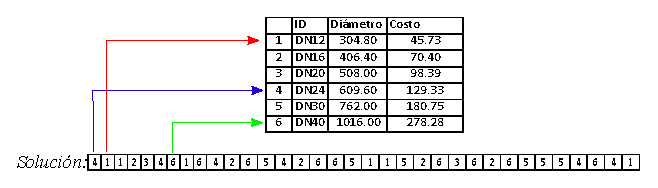
\includegraphics[width=\textwidth]{assets/Anexo/representacion_solucion_monoobjetivo.eps}
        \end{figure}

    \end{frame}

    \begin{frame}
        \frametitle{Representación de la solucion problema operacional}
        Problema de operación basado en el Régimen de bombeo.
        \begin{figure}
            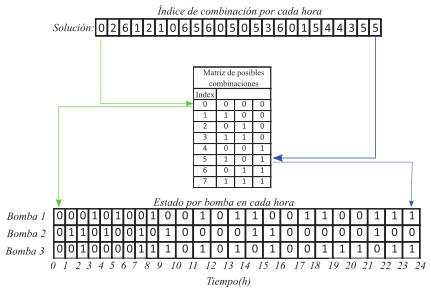
\includegraphics[scale=0.3]{assets/Anexo/representacion_solucion_multiobjetivo.eps}
        \end{figure}

    \end{frame}


\end{document}